\chapter{Background}
\label{cha:background}

\section{Cellular automata}

The \acf{CA} was originally proposed by Stanislaw Ulam and John Von
Neumann in the 1940s as a model of the growth of crystals and an attempt at
constructing a self-replicating system \cite{von_neumann_theory_1966}.

It is usually defined on a regular lattice in one or two dimension. Each of its
components is called a cell, and can be in a state $k \in \mathcal{S}$.

A neighborhood
function $\boldsymbol{N}$ is defined which associates each cell with its
neighbors on the lattice.
In general, a \ac{CA} can be constructed on any space $\mathcal{L}$ where such a function
can be defined. The space $\mathcal{L}$ specifies an indexing and the relation between the
cells. In practice, regular finite or infinite grids are chosen, $\mathcal{L} \subset \mathbb{Z}$ or
$\mathcal{L} \subset \mathbb{Z}^{2}$. For example, the grid could be a 1-dimensional torus with 10 cells,
that is $\mathcal{L}_{{T_{10}}} = \{1, 2, \ldots, 10 \}$. The neighborhood function has the
form
\begin{equation}
  \begin{aligned}
\boldsymbol{N}_{\mathcal{L}} :\quad & \mathcal{S} \rightarrow \mathcal{S}^{s}\\
&c_{i} \mapsto [c_{j}]_{j\in \mathcal{N}_{c_{i}}}
  \end{aligned}
\end{equation}
where $\mathcal{N}_{c_{i}}$ is the neighborhood of cell $c_{i}$, $s$ is the number of
cells in the neighborhood and the returned value is a finite set of cells, the
neighbors of cell $c_{i}$. For the torus $\mathcal{L}_{T_{10}}$ above, we can define the
neighbors to be the cell itself and the two immediately adjacent cells. This
type of 1D neighborhood is illustrated on Figure \ref{fig:1d_neigh}. It
corresponds to the following neighborhood function:
\begin{equation}
  \begin{aligned}
\boldsymbol{N}_{\mathcal{L}_{T_{10}}} :\quad & \mathcal{S} \rightarrow \mathcal{S}^{3} \\
&\boldsymbol{N}_{\mathcal{L}_{T_{10}}}(c_{i}) = \begin{cases}
                      [c_{i - 1}, c_{i}, c_{i + 1}],& \text{if}\quad i \in \{2,\ldots , 9\}\\
                       [c_{10}, c_{1}, c_{2}], & \text{if} \quad i = 1 \\
                       [c_{9}, c_{10}, c_{1}], & \text{if} \quad i = 10. \\
                    \end{cases}
  \end{aligned}
\end{equation}

On two dimensional grids, there are multiple ways to define the neighborhood.
Some common examples are the Moore neighborhood (see Figure \ref{fig:moore}) and
the Von Neumann neighborhood (see Figure \ref{fig:von_neumann}). In the rest we
omit the subscript on the neighborhood function $\boldsymbol{N}$ as we almost
always work with regular grids.

\begin{figure}[htbp]
  \centering
  \begin{subfigure}[c]{.3\linewidth}
    \centering
    
\includegraphics[width=\linewidth]{figures/1d_neigh}
    \caption{Standard 1D \ac{CA} neighborhood}
    \label{fig:1d_neigh}
  \end{subfigure}
  \begin{subfigure}[c]{.3\linewidth}
    \centering
    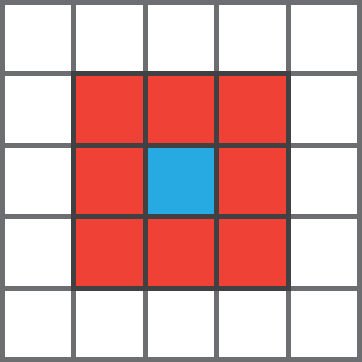
\includegraphics[width=\linewidth]{figures/moore}
    \caption{Moore neighborhood}
    \label{fig:moore}
  \end{subfigure}
  \begin{subfigure}[c]{.3\linewidth}
    \centering
    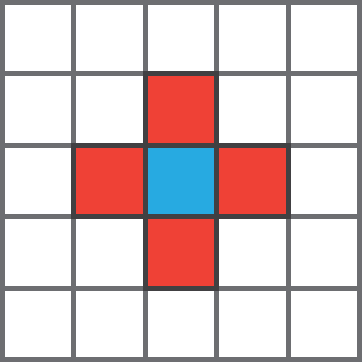
\includegraphics[width=\linewidth]{figures/von_neumann}
    \caption{Von Neumann neighborhood}
    \label{fig:von_neumann}
  \end{subfigure}

  \caption{Illustration of commonly used neighborhoods for 1D and 2D cellular automata.}
  \label{fig:neighborhoods}
\end{figure}

A \ac{CA} evolves in discrete time steps. An update rule $\boldsymbol{\Phi}$
defines the new state of a cell as a function of its local neighborhood at the
current time step. It is applied in parallel to all the cells. For a cellular
automaton in its initial state at time step 0 --- \ie a set of cells
$\left(c_{i}^{(0)}\right)_{i \in \mathcal{L}} \in \mathcal{S}^{|\mathcal{L}|}$, and a neighborhood function
$\boldsymbol{N}$, we have the following update rule
\begin{equation}
\begin{aligned}
\forall i \in \mathcal{L}, \quad c_{i}^{(t + 1)} = \boldsymbol{\Phi}\left(\boldsymbol{N}\left(c_{i}^{(t)}\right)\right)
\end{aligned}
\end{equation}

The details of an example update step on a 1 dimensional \ac{CA} is shown on
Figure \ref{fig:ca_base}. The neighborhood of the cell $c_{i}$ is itself and the
two immediately adjacent cells.

\begin{figure}[htbp]
  \centering
 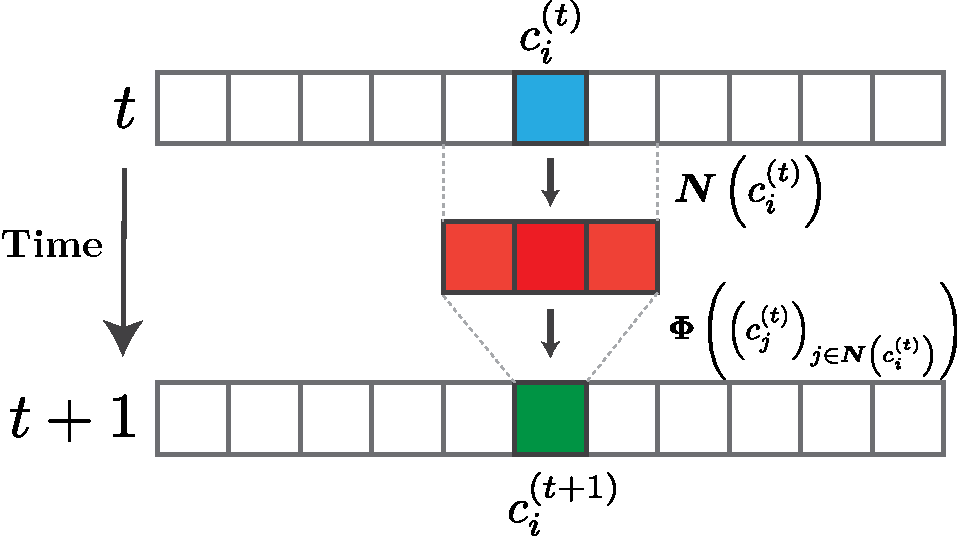
\includegraphics[width=.7\linewidth]{figures/ca_base}
  \caption{Illustration of a \acl{CA} update rule in 1 dimension. For each cell,
  we look up the neighboring cells and update its state according to the current
state of the neighbors.}
  \label{fig:ca_base}
\end{figure}

The function $\boldsymbol{\Phi}$ is often called a \emph{rule table} because it
associates an output state for each combinations of input neighbor states. These
output states can be looked up from a table containing all possible transitions
from inputs to outputs.

\paragraph{Rule representation}
A useful rule representation is obtained by listing all output state
corresponding to input configurations in a predetermined order. This results in
a list of values $[o_1, \ldots, o_{s^{|\mathcal{S}|}}]$, with $\forall i,\ o_{i} \in \mathcal{S}$, where $s$ is
the number of cells in a neighborhood, $\mathcal{S}$ is the space of available states and
$|\mathcal{S}|$ is the number of available states per cell. Using the $o_{i}$ as the
digits of a base-$|\mathcal{S}|$ number, each rule is uniquely represented by a number.

\paragraph{Boundary conditions}

A large number of variants of \acp{CA} have been constructed, modifying or
constraining various part of the definition above. We list some of them here.

\subsection{Elementary cellular automata}
\Acp{ECA} are the 1 dimensional \acp{CA} with two states per cell and
neighborhood size 3 --- the cell and its neighbors. There are 8 possible
configurations of a neighborhood with 3 cells and 2 states per cell, which
corresponds to 256 possible ways to define an \ac{ECA}. This small number of
rules enables exhaustively exploring the rule space and mapping out the \ac{ECA}
properties.

\cite{wolframNewKindScience2002, hudcovaClassificationComplexSystems2020,
  hudcovaComputationalHierarchyElementary2021}

\subsection{Asynchronous cellular automata}
A cellular automaton is said to be asynchronous when its cells are not all
updated in parallel at each time step. Several cell update schemes can
be chosen. Contrary to regular cellular automata, the grid has to be finite
because for an update rule to exist.

\subsection{Stochastic cellular automata}
In a stochastic cellular automaton, the update function $\boldsymbol{\Phi}$ is stochastic

\subsection{Discrete}
\subsection{Continuous}

\section{Reservoir computing}
